\documentclass[../../thesis.tex]{subfiles}


\newcommand{\rbV}{\ensuremath{\mathbb{V}}}
\newcommand{\rbVT}{\ensuremath{\rbV^T}}
\newcommand{\epspod}{\ensuremath{\varepsilon_\text{POD}}}

\newcommand{\inner}[2]{\left<#1, #2\right>}
\newcommand{\alemap}{\ensuremath{\mathcal{A}}}
\newcommand{\dt}{\ensuremath{\Delta t}}
\newcommand{\pexp}{\ensuremath{\frac{2\gamma}{\left(\gamma-1\right)}}}
\newcommand{\aleX}{\ensuremath{\mathcal{X}}}
\newcommand{\Ah}[1]{\ensuremath{\vb{#1}^{n+1}_h}}
\newcommand{\Ahm}[1]{\ensuremath{\vb{#1}^{m, n+1}_h}}
\newcommand{\Ahn}[1]{\ensuremath{\vb{#1}^{n}_h}}

\begin{document}

\section{(Hyper) Reduced Order Model}
\label{sec:rom_definition}
For any unseen parameter value, our aim is to be able to assemble and solve a smaller algebraic problem, 
and yet to obtain a solution close enough to that of the FOM.
% We present now the formulation for the Reduced Order Model (ROM).
In order to do so, first we need to obtain certain algebraic structures which capture the essence of the problem at hand.

% Offline phase
We do so by sampling the original problem at certain parameter values and processing snaphsots of the solution and the operators, obtained from the solution of the FOM problem.
This is called the \emph{offline phase}.
% Online phase
Later on, we exploit these static structures to build reduced operators which capture the dynamics of the problem sufficiently well, solve a smaller algebraic system and then recover the solution in the original mesh variables, in order to postprocess it.
This is called the \emph{online phase}.

% Then, we should be able to map back the solution to the original dimension $N_h$, since it is the geometrical space where solution plots on the original mesh are meaningful. 

We will use the Reduced Basis Method (RB) to construct an ad-hoc problem-based basis to represent our ROM;
the Discrete Empirical Interpolation Method (DEIM) and its matrix version (MDEIM) 
to build suitable approximations of the algebraic operators involved. 

The continuous reduced problem formulation is skipped since it will not be used. 
% For completeness, it will be defined in the appendix along with relevant remarks.
Therefore, we jump directly into the discrete problem.
We recall that we are focused on reducing the problem for 
the homogeneous component $\hat{u}(x)$ of our solution, 
that is, for the weak formulation given by 
the system of equations~\eqref{eq:1d_fom_weak_formulation_homogeneous}.  

% -----------------------------------------------------------------------------
\subsection{A Naive Approach}
We have included in the title the word \emph{naive} 
because we will define the reduction problem in a very blunt way,
where many ineffiencies will show up.
We do so to motivate the operator reduction procedures we will include later on.

In the reduced context, we use a finite space $V_N \subset V_h$, where we can represent the solution as the linear combination of a set of orthonormal\footnote{If they were not, we can always make them so via Gram-Schmidt.} \mbox{problem-based} basis functions~$\psi_i(x)$,
\begin{equation}
    \hat{u}_N(x) = \sum_j^{N} \hat{u}_{N_j} \psi_j(x).
    \label{eq:1d_rom_burgers_rb_expansion}
\end{equation}
Their goal is to capture the problem dynamics, so these RB solution modes~$\psi_i(x)$ have global support.
Since we want to reduce the number of modes we need to represent our solution, we usually expect or desire to have $N \ll N_h$, . 

To maintain focus and in favor of generality, let us assume at this point that the global basis functions are given, and that they are zero at the boundary.
We will give details on how to obtain them later on.

\subsubsection{Reduced Space Projection}
Since we can represent any function in terms of our FE basis functions~$\varphi_i(x)$, 
we have a linear mapping between the problem-based functions~$\psi_j(x)$ and the nodal basis functions.
This allows us to establish the following relation between the problem solution in the reduced and original spaces,
\begin{equation}
    \label{eq:1d_rom_burgers_projection_relation}
    \vb{\hat{u}}_h = \rbV \vb{\hat{u}}_N.
\end{equation}
The entries of the $\rbV$ matrix represent the coefficients of the global basis representation in the FE basis, 
% Each column of $\mathbb{V}$ represents the projection of the problem-based function $\psi_i(x)$ in terms of all the nodal basis functions $\varphi_j(x)$,
\begin{equation}
    \psi_i(x) = \sum_j \left[\mathbb{V}\right]_{ji}\varphi_j(x).
\end{equation}

% -----------------------------------------------------------------------------
\subsubsection{Discrete Reduced Problem Assembly}
In theory, to assemble the reduced problem operators, 
one could actually compute the inner products defined in Equations~\eqref{eq:1d_fom_linear_system_operators} 
with these new basis functions $\psi_i(x)$.
In practice, it is more convenient to project the algebraic FOM operators with \mbox{matrix-matrix} and \mbox{matrix-vector} products into the reduced space, 
\begin{subequations}
    \label{eq:1d_rom_linear_system_operators}
    \begin{align}
        \vb{X}_{N}^{n+1}       &= \rbVT \vb{X}_{h}^{n+1} \rbV, \\
        \vb{F}_{N}^{n+1}       &= \rbVT \vb{F}_{h}^{n+1}, 
        % \vb{M}_{N}^{n+1}       &= \rbVT \vb{M}_{h}^{n+1} \rbV, \\
        % \vb{A}_{N}^{n+1}       &= \rbVT \vb{A}_{h}^{n+1} \rbV, \\
        % \vb{C}_{N}^{n+1}       &= \rbVT \vb{C}_{h}^{n+1} \rbV, \\
        % \vb{     N}_{N}^{n+1}  &= \rbVT \vb{     N}_{h}^{n+1} \rbV, \\
        % \vb{\hat{N}}_{N}^{n+1} &= \rbVT \vb{\hat{N}}_{h}^{n+1} \rbV, \\
        % \vb{F}_{N}^{n+1}       &= \rbVT \vb{F}_{h}^{n+1},  \\
        % \vb{F}_{{g,N}}^{n+1}   &= \rbVT \vb{F}_{{g,h}}^{n+1},
    \end{align}
\end{subequations}
where $\vb{X}_{h}$ and $\vb{F}_{h}$ stand for each of the FOM operators (matrices and vectors respectively).
The assembly of matrices based on a FE basis can be easily done in parallel due to their local support, 
whereas the integration of functions with global support is not necessarily computationally efficient.


By doing so, we find the following pure ROM problem for the time evolution problem,
\begin{subequations}
    \label{eq:1d_rom_weak_formulation_discrete}
    \begin{align}
        m_{\text{BDF}} \vb{M}^{n+1}_{N} \vb{\hat{u}}_{N}^{n+1}
        + \dt \vb{C}^{n+1}_{N} \vb{\hat{u}}_{N}^{n+1}
        + \dt \vb{A}^{n+1}_{N} \vb{\hat{u}}_{N}^{n+1}
        \nonumber 
        \\[2mm]
        + \dt \vb{\hat{N}}^{n+1}_{N} \vb{\hat{u}}_{N}^{n+1}
        + \dt \left[\vb{N}^{n+1}_{N}\left(\vb{\hat{u}}_{N}^{*}\right)\right] \vb{\hat{u}}_{N}^{n+1}
        \nonumber
        \\[2mm]
        = \vb{F}_{\vb{\hat{u}}_{N}}^{n}
        + \dt \vb{F}_{g,N}^{n+1},
        \\[2mm]
        \vb{\hat{u}}_N^{0} = \vb{\hat{u}}_{N,0}.
    \end{align}
\end{subequations}
% \begin{subequations}
%     \label{eq:1d_rom_weak_formulation_discrete}
%     \begin{align}
%         \vb{M}_N \vb{\hat{u}}_{N}^{n+1} + \Delta t \vb{A}_N \vb{\hat{u}}_{N}^{n+1} &= \vb{F}^{n}_{\vb{\hat{u}}_N} \\
%         &+ \Delta t \vb{F}_N^{n+1} + \Delta t \vb{F}^{n+1}_{g, N}, \nonumber \\
%         \vb{\hat{u}}_N^{0} &= \vb{\hat{u}}_{N,0}.
%     \end{align}
% \end{subequations}
If we collect terms and factor out the unknowns we get a linear system, 
this time in the reduced space, to be solved for each time step to advance the solution,
% \begin{subequations}
%     \label{eq:1d_rom_linear_system_timestep}
%     \begin{align}
%         \vb{K}_N^{n+1} \vb{\hat{u}}_N^{n+1} &= \vb{b}_N^{n+1}, \\
%         \vb{K}_N^{n+1} &= \vb{M}_{N}^{n+1} + \Delta t \vb{A}_{N}^{n+1}, \\
%         \vb{b}_N^{n+1} &= \vb{F}_{\vb{\hat{u}}_N}^{n} + \Delta t \vb{F}_N^{n+1} + \Delta t \vb{F}_{g,N}^{n+1}, \\
%         \vb{\hat{u}}_N^{0} &= \vb{\hat{u}}_{N,0}.
%     \end{align}
% \end{subequations}
\begin{subequations}
    \label{eq:1d_rom_linear_system_timestep}
    \begin{align}
        \vb{K}_{N}^{n+1} \vb{\hat{u}}_{N}^{n+1} &= \vb{b}_{N}^{n+1}, 
        \\
        \vb{\hat{u}}_{N}^{0} &= \vb{\hat{u}}_{N,0};
        \\[2mm]
        \vb{K}_{N}^{n+1} &= m_{\text{BDF}} \Ah{M} + \dt \left[\Ah{A} + \Ah{C} \right. 
        \nonumber 
        \\
                        &\left. + \Ah{\hat{N}} + \Ah{N}\left(\vb{\hat{u}}_{N}^{*}\right)\right],
        \\[2mm]
        \vb{b}_{N}^{n+1} &= \vb{F}_{\vb{\hat{u}}_{N}}^{n} + \dt \vb{F}_{g,N}^{n+1}.
    \end{align}
\end{subequations}
All of the previous has the same algebraic pattern as the FOM problem.
The only difference is the size of the operators, much smaller due to the small size of $N$. 

% -----------------------------------------------------------------------------
\subsubsection{ROM Time Discretization Forcing Term}
The forcing term $\vb{F}_{\vb{\hat{u}}_h}^{n}$ due to the time discretization has been intentionally left out in the previous section.
We could naively project it too, 
\begin{equation}
    \vb{F}_{\vb{\hat{u}}_N}^{N} = \rbVT \vb{F}_{\vb{\hat{u}}_h}^{n},
\end{equation}
but this would force us to reconstruct the FE vector of the ROM at each time-step, making the integration cumbersome.
To get around this issue, we can exploit the algebraic representation of $\vb{F}_{\vb{\hat{u}}_h}^{n}$, 
given in Equation~\eqref{eq:1d_fom_forcing_term_time_mass_matrix} in terms of the mass matrix. 
The forcing term due to the time discretization takes the following form in the ROM:
\begin{equation}
    \vb{F}_{\vb{\hat{u}}_N}^{n} = 
    \begin{cases}
        \vb{M}_{N}^{n+1} \vb{\hat{u}}_{N}^{n},                & \text{BDF-1},
        \\
        2 \vb{M}_{N}^{n+1} \vb{\hat{u}}_{N}^{n}
        - \frac{1}{2}\vb{M}_{N}^{n+1} \vb{\hat{u}}_{N}^{n-1}, & \text{BDF-2}.
    \end{cases}
\end{equation}
Again, these mimic the algebraic pattern obtained in the FOM.

% -----------------------------------------------------------------------------
\subsubsection{Boundary and Initial Conditions}
The computation of the initial condition~$\vb{\hat{u}}_{N,0}$ is to be done in two steps. 
First, the initial condition~$\vb{\hat{u}}_{h,0}$ in the FOM space needs to be computed as a FE vector via interpolation or projection.
% by means of the techniques explained in Section~\ref{sec:1d_fom_projection_interpolation}.
Then, this FE representation $\vb{\hat{u}}_{h,0}$ needs to be projected unto the reduced space. 
Since we are dealing with an orthonormal basis, we can use the matrix~$\rbV$ to project the FE vector departing from the \mbox{FOM-ROM} relation given in Equation~\eqref{eq:1d_rom_burgers_projection_relation},
\begin{equation}
    \rbVT \vb{\hat{u}}_{h,0} = \underbrace{\rbVT \rbV}_{\mathbb{I}} \vb{\hat{u}}_{N,0} 
    \rightarrow 
    \vb{\hat{u}}_{N,0} = \rbVT \vb{\hat{u}}_{h,0}.
\end{equation}

Regarding the spatial boundary conditions, at this point of the naive reduction scheme, two facts come into play, which we first present and then put together:
\begin{enumerate}
    \item The weak form has homogeneous boundary conditions.
    \item The ad-hoc RB solution modes~$\psi_i(x)$ are zero at the boundaries,
    \begin{equation*}
        \psi_i(x) = 0 \quad \forall \, x \in \partial \Omega.
    \end{equation*}
\end{enumerate}
These two facts imply that the projection of the operators, 
Equation~\eqref{eq:1d_rom_linear_system_operators}, 
does not break the original constraint of homogeneous boundary conditions;
and that the linear expansion of the solution~$\hat{u}_N(x)$ in the span of~$V_N$, 
Equation~\eqref{eq:1d_rom_burgers_rb_expansion}, 
is always true.

Once the reduced homogeneous solution~$\hat{u}_N(x)$ is obtained, 
it can be brought back to the original space~$V_h$ via 
Equation~\eqref{eq:1d_rom_burgers_projection_relation}, 
and then added to the FE representation of the Dirichlet lifting, 
to obtain the solution $u_h(t, \mu)$ in the physical domain,
\begin{equation}
    u(x, t; \mu) \simeq u_h(t, \mu) = \rbV \hat{u}_N(t, \mu) + g_h(t,\mu).
\end{equation}

% -----------------------------------------------------------------------------
\subsubsection{Naive Reduction Scheme: Final Remarks}
At this point, the naive reduction scheme for the RB-ROM has been defined and explained.
However, some aspects of it remain unattended.

The construction of the problem-based basis functions $\psi_i(x)$:
there are many methods to build them, and which combination of them we choose 
defines which reduction method we are applying, along with their advantages and requirements.

The \emph{offline-online decomposition}: 
that is, to uncouple the usage of FOM operators in as much as possible from the integration of the ROM. 
Ideally, no FOM structures should be assembled during the online phase.
In this naive scheme, we are clearly not meeting such requirement, 
since we need to assemble all the FOM operators and then project them \emph{for each time step}.

Hence, some additional sections need to be brought up, 
in order to complete our definition of the reduction scheme.
We now treat the construction of the basis functions, Section~\ref{sec:1d_rom_burgers_basis_construction}; and the approximation of the algebraic operators, Section~\ref{sec:1d_rom_burgers_system_approximation_deim}.

% -----------------------------------------------------------------------------
\subsection{Reduced Basis Construction}
\label{sec:1d_rom_burgers_basis_construction}
Hereby we layout the details of the basis construction, that is, the definition of the $\psi_i(x)$ functions.
There are many techniques to build such basis.
We opt for an automatic and out-of-the-box technique: the nested POD approach
\cite{Santo_Manzoni_2019}. 

On paper, the most simple basis anyone could come up with is 
a collection of solution snaphsots for different parameter values and time steps, 
\begin{align}
    \Psi_{\hat{u}} &:= [\psi_i] \nonumber \\
    &= [\hat{u}_h(t^0; \mu_0), \hat{u}_h(t^1; \mu_0), 
    \ldots, \hat{u}_h(t^j; \mu_i), \ldots], \nonumber \\
    &= [\Psi_{\hat{u}}(\mu_0), \Psi_{\hat{u}}(\mu_1), \ldots, \Psi_{\hat{u}}(\mu_{N_{\mu}})]
\end{align}
Yet, this basis $\Psi_{\hat{u}}$ is unpractical from a computational point of view: we could not possibly store all the basis vectors or compute efficiently all the required algebraic operations with them.
Additionally, it would probably lead to ill-posed linear systems, since the vectors are almost linearly dependent. 

However, since all these vectors arise from the same PDE (although for different parametrizations of it), and for each time step the solution is close to the previous one, in a way, we could expect there to be a lot of repeated information inside each $\Psi_{\hat{u}}(\mu_i)$, and consequently, inside $\Psi_{\hat{u}}$.
We can exploit this fact by using a compression algorithm, such as the Proper Orthogonal Decomposition (POD), to find a set of vectors which sufficiently capture the span of $\Psi_{\hat{u}}$, and yet do so with less basis vectors. 

% We call this the \emph{method of snapshots}. 

% -----------------------------------------------------------------------------
\subsubsection{POD Space Reduction}
\label{sec:1d_rom_burgers_basis_construction_pod}
% We can see the Proper Orthogonal Decomposition (POD) as 
% an enhanced Gram-Schmidt orthonormalization procedure: not only an orthonormal basis is obtained, 
% but additionally the output basis vectors recover hierarchically the span of the original space 
% given by the input vectors.
We define the $POD: X \rightarrow Y$ function between two normed spaces, 
such that $Y \subseteq  X$, 
which takes as inputs a collection of~$N_S$ vectors $y_k \in X$,
a prescribed tolerance error $\epspod$,
\begin{equation}
    [\psi_i]_{i=1}^{N_{POD}} = POD\left([y_k]_{k=1}^{N_S}, \epspod\right).
\end{equation}
and returns a basis of modes $\psi_i \in Y$ to approximate the span of $y_k$.
This function returns a collection of orthonormal $N_{POD}$ vectors, whose span is a subset of the input vector span.
The modes $\psi_i$ are obtained from an optimality problem in the $L^2$ norm,
\begin{equation}
    (v_i, \psi_i) \, \text{s.t.} \, \min \sum_k \norm{y_k(x) - \sum_i v_i \psi_i}^2 \leq \epspod,
\end{equation}
that is, the representation of any vector in the original space can be reconstructed the POD basis, 
and the error in the $L^2$ norm should be less or equal to \epspod.

There is a relation between the prescribed tolerance error $\epspod$ 
and the outcoming number of modes $N_{POD}$, 
\begin{equation}
    N_{POD} = N_{POD}(\epspod).
\end{equation}
This function usually shows exponential decay, or a sharp drop beyond a given number of modes.
If a problem can be reduced, beyond a given number of modes, 
including more in the approximation will not improve significantly the approximation error.

% Alternatively to a prescribed error, one could directly ask for a prescribed number of basis functions~$N^{*}_{POD} \leq N_S$,
% \begin{equation}
%     [\psi_i]_{i=1}^{N^{*}_{POD}} = POD\left([\varphi_i]_{i=1}^{N_S}, N^{*}_{POD}\right).
% \end{equation}

% -----------------------------------------------------------------------------
\subsubsection{Nested POD Basis Construction}
\label{sec:1d_rom_burgers_basis_construction_nested}
% A simple procedure to leverage the compression properties of the POD function, 
% and the nested structure of our PDE with respect to time and the parameters; 
We now describe the nested POD algorithm, 
sketched in Figure~\ref{fig:treewalk_sketch}.
\begin{figure}[h]
    \centering
    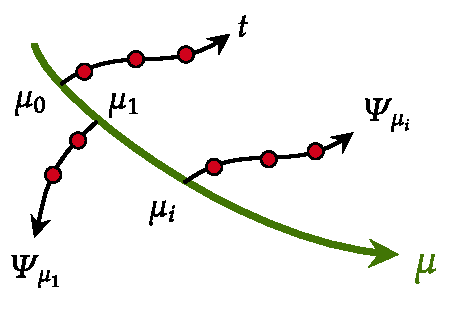
\includegraphics[width=0.8\columnwidth]{research_project/piston/figures/treewalk.pdf}
    \caption{Nested POD treewalk.
    For each parameter $\mu$ a simulation is run,
    and snaphsots are collected and compressed in time (red dots).
    This provides a collateral basis for each value of the parameter.
    These bases are finally compressed into one, 
    which summarizes the changes in time and parameters.}
    \label{fig:treewalk_sketch}
\end{figure}
First, for a fixed parameter value, we build a POD basis from the snapshots at different time steps,
\begin{align*}
    \Psi_{\mu_0} &= POD_{\varepsilon}\left(\left[\hat{u}_h(t^0; \mu_0), \ldots, \hat{u}_h(t^T; \mu_0)\right]\right), \\
    \Psi_{\mu_1} &= POD_{\varepsilon}\left(\left[\hat{u}_h(t^0; \mu_1), \ldots, \hat{u}_h(t^T; \mu_1)\right]\right), \\  
    \ldots, \\
    \Psi_{\mu_{N_{\mu}}} &= POD_{\varepsilon}\left(\left[\hat{u}_h(t^0; \mu_{N_{\mu}}), \ldots, \hat{u}_h(t^T; \mu_{N_{\mu}})\right]\right).
\end{align*}
Then, all the $\mu$-fixed POD basis 
(which sum up the information contained in the time evolution direction), 
are compressed again using a POD,
\begin{equation*}
    \rbV := \Psi = POD_{\varepsilon} \left(\left[\Psi_{\mu_0}, \Psi_{\mu_1}, \ldots, \Psi_{\mu_{N_{\mu}}}\right]\right).
\end{equation*}
In the end, we obtain a basis $\Psi = [\psi_i] = \rbV$, 
which contains information for parameter variations and time evolution.
%It has been built in a computationally efficient manner, 
This leads to an efficient basis, in terms of storage and numerical stability
Different error tolerances could be prescribed at the time and parameter compression stages
for demanding\footnote
{
    Ideally, the whole POD basis is stored and then
    partially loaded during the online stage,
    according to the desired ROM accuracy.
    However, the offline stage might still be a memory-consuming one,
    which could require triming at runtime the POD basis before storing it.
} problems.

We call this an automatic and out-of-the-box procedure 
because it does not require further developments 
beyond the storage of the snapshots and the implementation of the POD algorithm.
It only requires the construction of a collection of parameter values to solve for.
This can be done with random sampling techniques, 
or if some physical knowledge is available, 
a custom selection of parameter subsets for which the solution will present strong variations 
(leading to the identification of richer RB solution modes).

Since we are using an SVD-based POD, we need to set a threshold for
the acceptable singular values/modes.
We set this threshold at $10^{-7}$,
since after visual inspection of the resulting modes revealed
numerical noise beyond this figure.
% Naturally, more involved procedures exist to create the final basis $\Psi$, 
% but they need the capacity to evaluate how accurately or poorly 
% is the basis performing at capturing the problem dynamics.
% This can be dealt with the determination of sharp \emph{a priori} error estimators,
% but that again requires theoretical developments 
% (which we value deeply but consider out of our range at the moment).

% We leave this for later.

% -----------------------------------------------------------------------------
\subsection{(M)DEIM: System Approximation}
\label{sec:1d_rom_burgers_system_approximation_deim}
During the offline stage (where the FOM problem is solved), 
we have to assemble all the discrete operators for each time step;
during the online stage we additionally have to project them 
onto the reduced space as well, 
as shown in Equations~\eqref{eq:1d_rom_linear_system_operators}.
This projection step can mean a ROM is still costly,
if it only relies on RB solution modes to reduce the problem.
This will be our main motivation to include a system approximation technique,
with the goal of speeding up the construction of the operators.

An essential ingredient for our system approximation is the concept of \emph{parameter and time separable} problems 
(or the existence of an \emph{affine decomposition}).
This takes place when the spatial operators (bilinear or linear forms)
present the following functional separable form:
\begin{equation}
    \label{eq:1d_rom_burgers_separable_form_time_param}
    A_h(t, \mu) = \sum_q^{Q_a} \Theta_q^a(t, \mu) A_{h,q},
\end{equation}
where the coefficient functions are real-valued, \mbox{$\Theta_q^a(t, \mu) \in \mathbb{R}$};
and the RB operator modes $A_{h,q}$ are parameter-independent.

This expansion can be used for both matrices or vectors provided 
the topology of the mesh does not change.
If this is the case, the matrices can be transformed into vectors
by stacking the columns\footnote{We used a CSR storage format.}, 
and later on brought back to matrix form once any necessary operation has been carried out.

If we had such a decomposition, once we had computed the basis matrix \rbV, 
we could project each mode of the operator basis $A_{h, q}$ to obtain an expression for the reduced operator, 
\begin{equation}
    \begin{split}
        A_N(t, \mu) &= \rbVT A_h(t, \mu) \rbV,
        \\ 
        &= \sum_q^{Q_a} \Theta_q^a(t, \mu) \rbVT  A_{h, q} \rbV, 
        \\
        A_N(t, \mu) &= \sum_q^{Q_a} \Theta_q^a(t, \mu) A_{N,q}.
    \end{split}
\end{equation}
Since $A_{N, q}$ is fixed, provided that we had a way to evaluate each $\Theta_q^a(t, \mu)$, 
we would be able to build the reduced operator for a given parameter for each time step without having to use any FOM operator. 

% -----------------------------------------------------------------------------
\subsubsection{Discrete Empirical Interpolation Method}
Naturally, not many problems are likely to present a separable form as the one shown above.
Even a simple linear heat equation problem, due to the time-deformation of the mesh, cannot be presented in such a form. 

To tackle this issue, we use the Discrete Empirical Interpolation Method (DEIM).
This method is a numerical extension of its analytical sibling, the Empirical Interpolation Method (EIM).
Basically, it mimicks the idea of creating a basis for the solution space, but this time centered around the operator space.
By means of a nested POD as we explained in Section~\ref{sec:1d_rom_burgers_basis_construction_nested}, 
if we replace the solution snapshots with operator snapshots, 
we can build the static and problem-dependent basis $A_{h,q}$.

Since we will be creating the operator basis with an approximation technique, 
an error is expected in the reconstruction of the actual operator, 
and so we introduce the notation $A_h^m(t, \mu)$ to reference the approximation of the operator via the (M)DEIM algorithm,
\begin{equation}
    \label{eq:1d_rom_burgers_system_approximation}
    A_h(t, \mu) \simeq A_h^m(t, \mu) = \sum_q^{Q_a} \Theta_q^a(t, \mu) A_{h,q}.
\end{equation}
Naturally, this idea leads to the concept of approximated reduced operators,
\begin{equation}
    A_N(t, \mu) \simeq A_N^m(t, \mu) = \sum_q^{Q_a} \Theta_q^a(t, \mu) A_{N,q},
\end{equation}
which is the approximation of the reduced operators when the collateral basis 
has been projected unto the reduced space.

% -----------------------------------------------------------------------------
\subsubsection{Evaluation of the Coefficient Functions}
To evaluate the $\Theta_q^a(t, \mu)$ functions, we set and solve an interpolation problem;
that is, we enforce the approximation to actually match certain entries of the operator, 
\begin{equation}
    \begin{split}
        [A_h(t, \mu)]_{k} &= [A_h^m(t, \mu)]_{k} \\
                          &= \sum_q^{Q_a} \Theta_q^a(t, \mu) [A_{h, q}]_{k}, 
    \end{split}
    \label{eq:1d_rom_burgers_interpolation_problem}
\end{equation}
for certain indices~$k \in \mathcal{I}_a$ such that~$\left|\mathcal{I}_a\right| = Q_a$.
These indices $\mathcal{I}_a$ are known as the reduced mesh nodes, 
sketched in Figure~\ref{fig:reduced_mesh}.
\begin{figure}[h]
    \centering
    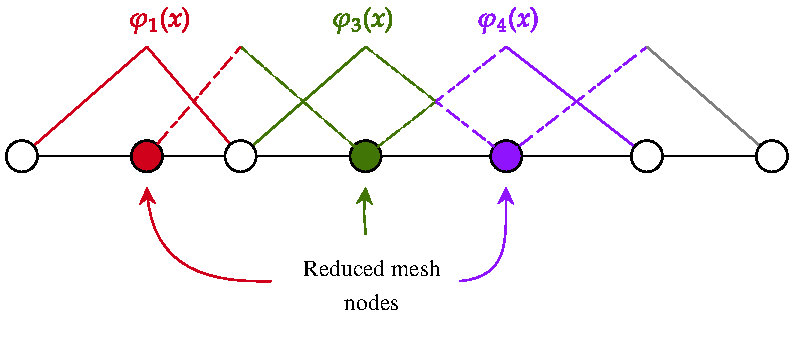
\includegraphics[width=0.90\columnwidth]{research_project/piston/figures/reduced_mesh_nodes.pdf}
    \caption{Reduced mesh nodes $\mathcal{I}_a$ sketch 
    for $\mathbb{P}1$ Lagrangian finite element basis functions. 
    The weak form integral evaluation only takes place for a restricted subset of mesh elements,
    to assemble the entries corresponding to the selected nodes.  
    In dashed are shown the interactions with adjacent finite elements basis functions.
    A sketch for a 2D domain can be found in \cite{2015_efficientModelReductionParametrizedSystemsMatrixDeim_Negri}.}
    \label{fig:reduced_mesh}
\end{figure}
The notation $[A_h(t, \mu)]_{k}$ stands for the value of the operator at the given mesh node $k$.
In the FE context it can be obtained by integrating the weak form locally.

This leads to a determined system, where each $\Theta_q^a(t, \mu)$ is unknown.
The indices $\mathcal{I}_a$ are selected during the offline stage, 
according to error reduction arguments of the reconstruction error
\cite{2010_nonlinearModelReductionDeim_chaturantabut},
\begin{equation}
    e_a(t, \mu) = \norm{A_h(t, \mu) - A_h^m(t, \mu)}.
\end{equation}

\newpage
% -----------------------------------------------------------------------------
\subsubsection{Reduction of the Trilinear Term}
We recall that the trilinear operator $N_h(u^{*})$ 
from Equation~(\ref{eq:trilinear_weak_form})
takes as input in its first argument an extrapolation of the velocity $u^{*}$.
This extrapolation lives in the same function space as the solution:
from Equation~(\ref{eq:u_star_approximation}),
it is a linear combination of past discrete timestamps.

% This would allow us to span a larger parameter space,
% potentially larger than the one used to identify the RB solution modes.
Therefore, two approaches can be followed to build the the trilinear operator modes,
\begin{itemize}
    \item (\mbox{$u^{*}$-general}) collecting the snapshots from the FOM simulation \cite{Santo_Manzoni_2019};
    \item (\mbox{$u^{*}$-restricted}) collecting the snapshots from evaluations of the operator with RB solution modes.
\end{itemize}
The first approach to simply 
collect and compress the operator snapshots 
during the offline phase of the FOM,
with the general nested POD algorithm described 
in Section~\ref{sec:1d_rom_burgers_basis_construction_nested}.
This would tie the operator snapshots to the parameter space
sampled to identify the RB solution modes.

The second approach is to recognise that in the execution of the ROM,
the first component of the trilinear term, the extrapolated solution, 
will always be expressed in the finite-dimensional subspace of the RB solution modes
(as by Equation~(\ref{eq:1d_rom_burgers_rb_expansion})).
Thus, why not use these modes to assemble the operator snapshots?
Both approaches are summarized in Table~\ref{tab:summary_trilinear_strategies}.

The \mbox{$u^{*}$-restricted} strategy requires a slight modification of the nested POD algorithm.
Instead of two, we have three nested levels: 
parameters, modes and time, as sketched in Figure~\ref{fig:treewalk_trilinear_sketch}.
\begin{figure}[h]
    \centering
    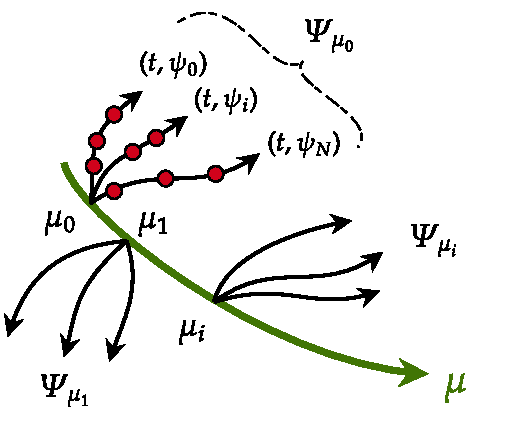
\includegraphics[width=0.8\columnwidth]{research_project/piston/figures/treewalk-trilinear.pdf}
    \caption{Nested POD treewalk for the trilinear term, 
    \mbox{$u^{*}$-restricted} strategy.
    The parameter space is sampled, for each parameter value and RB solution mode 
    snaphsots are collected and compressed in time (red dots).
    This provides a collateral basis for each parameter.
    These bases are finally compressed into one, 
    which summarizes the changes in time, parameters and RB solution modes.}
    \label{fig:treewalk_trilinear_sketch}
\end{figure}

We set a parameter, we pick a mode, collect as many snapshots
as time steps, and compress:
\begin{equation}
    \Psi_{\mu_i, \psi_0} = POD(\qty{N^{n}_h(\psi_0)}^{n=T}).
\end{equation}
This gives us a basis for the parameter/mode tuple $\Psi_{\mu_i, \psi_0}$. 
Then we pick the next mode, and obtain a basis for it, $\Psi_{\mu_i, \psi_1}$.
So on and so forth, we get as many bases as modes for that given parameter.
We then compress thoses bases altogether to obtain one final parameter basis,
\begin{equation}
    \Psi_{\mu_i} = POD(\qty{\Psi_{\mu_i, \psi_j}}^{j=N}),
\end{equation}
which collects the effects of each mode and time variation (for that specific parameter).
We repeat the process again for another parameter, 
until we end up with one operator basis,
which is the result of compressing all parameter bases,
\begin{equation}
    \Psi_{N_h} = POD(\qty{\Psi_{\mu_i}}^{i=N_{\mu}}).
\end{equation}
An advantage of this procedure is that it can be used when 
the FOM simulation is not available, 
e.g. when the RB solution modes are obtained from experimental data.

\begin{table}[h]
    \centering
    \caption{Trilinear operator N-MDEIM reduction approaches.
    \\
    The snapshots outset ("Op. assembly"), 
    the first argument of the weak form ("1st argument"),
    and the treewalk pattern are compared.
    \\
    The restricted strategy has an additional nesting level, 
    but it can be run as an independent step during the offline stage
    (provided that the RB solution modes are given).}
    \begin{tabular}{@{}lccc@{}}
    \toprule
                       & Op. assembly   & 1st argument          & Treewalk                                   \\ \midrule
    $u^{*}$-general    & FOM simulation & Extrapolation $u^{*}$ & Figure~\ref{fig:treewalk_sketch}           \\
    $u^{*}$-restricted & Ind. offline step      & RB solution modes     & Figure~\ref{fig:treewalk_trilinear_sketch} \\ \bottomrule
    \end{tabular}
    \label{tab:summary_trilinear_strategies}
\end{table}

% -----------------------------------------------------------------------------
\subsection{Hyper Reduced Order Model}
With an approximation of the reduced operators available, 
we can define yet another algebraic problem to integrate and 
obtain the reduced solution in time for a given parametrization,
\begin{subequations}
    \label{eq:1d_hrom_weak_formulation_discrete}
    \begin{align}
        m_{\text{BDF}} \vb{M}^{m, n+1}_{N} \vb{\hat{u}}_{N}^{m, n+1}
        + \dt \vb{C}^{m, n+1}_{N} \vb{\hat{u}}_{N}^{m, n+1}
        \nonumber 
        \\ 
        + \dt \vb{A}^{m, n+1}_{N} \vb{\hat{u}}_{N}^{m, n+1}
        \nonumber 
        \\ 
        + \dt \vb{\hat{N}}^{m, n+1}_{N} \vb{\hat{u}}_{N}^{m, n+1}
        \nonumber 
        \\ 
        + \dt \left[\vb{N}^{m, n+1}_{N}\left(\vb{\hat{u}}_{N}^{n}\right)\right] \vb{\hat{u}}_{N}^{m, n+1}
        \nonumber
        \\
        = \vb{F}_{\vb{\hat{u}}_{N}}^{m, n}
        + \dt \vb{F}_{g,N}^{m, n+1};
        \\
        \vb{\hat{u}}_N^{0} = \vb{\hat{u}}_{N,0}.
    \end{align}
\end{subequations}
If we collect terms and factor out the unknowns we get a linear system, 
in the reduced space and with approximated operators, 
to be solved for each time step to advance the solution,
\begin{subequations}
    \label{eq:1d_hrom_linear_system_timestep}
    \begin{align}
        \vb{K}_{N}^{m, n+1} \vb{\hat{u}}_{N}^{m, n+1} &= \vb{b}_{N}^{m, n+1}, 
        \\
        \vb{\hat{u}}_{N}^{0} &= \vb{\hat{u}}_{N,0};
        \\[5mm]
        \vb{K}_{N}^{m, n+1} &= m_{\text{BDF}} \Ahm{M} + \dt \left[\Ahm{A} + \Ahm{C} \right. 
        \nonumber 
        \\
                        &\left. + \Ahm{\hat{N}} + \Ahm{N}\left(\vb{\hat{u}}_{N}^{m, *}\right)\right],
        \\[2mm]
        \vb{b}_{N}^{m, n+1} &= \vb{F}_{\vb{\hat{u}}_{N}}^{m,n} + \dt \vb{F}_{g,N}^{m, n+1}.
    \end{align}
\end{subequations}
Each of the operators present in the problem will have associated 
an operator basis and will require the solution of 
the interpolation problem \eqref{eq:1d_rom_burgers_interpolation_problem} 
for each time step and parameter value.
Although this could still seem like a costly procedure, 
if the operators are actually reduceable, 
the number of basis functions $Q_m, Q_a, Q_f, Q_{f,g}$ should be small,
and thus way simpler problems than assembling the whole operator and 
then carrying out the projection.

% Note that the vector $\vb{F}_{\vb{\hat{u}}_N}^{n}$ is not approximated.
% The projection of the previous solution is directly obtained in the reduced space.

Once the reduced homogeneous solution $\hat{u}^{m}_N(x)$ is obtained 
with approximated operators, it can be brought back to the original space $V_h$ 
via Equation~\eqref{eq:1d_rom_burgers_projection_relation}, 
and then added to the Dirichlet lifting, 
to get the solution in the physical domain,
\begin{equation}
    u(x, t; \mu) \simeq u_h^{m}(t, \mu) = \rbV \hat{u}^{m}_N(t, \mu) + g_h(t,\mu).
\end{equation}

\end{document}


